% Judul dokumen
\title{Buku Tugas Akhir ITS}
\author{Musk, Elon Reeve}

% Pengaturan ukuran teks dan bentuk halaman dua sisi
\documentclass[12pt,twoside]{report}

% Pengaturan ukuran halaman dan margin
\usepackage[a4paper,top=30mm,left=30mm,right=20mm,bottom=25mm]{geometry}

% Pengaturan ukuran spasi
\usepackage[singlespacing]{setspace}

% Pengaturan detail pada file PDF
\usepackage[pdfauthor={\@author},bookmarksnumbered,pdfborder={0 0 0}]{hyperref}

% Pengaturan jenis karakter
\usepackage[utf8]{inputenc}

% Pengaturan pewarnaan
\usepackage[table,xcdraw]{xcolor}

% Pengaturan kutipan artikel
\usepackage[style=numeric, backend=biber]{biblatex}

% Package lainnya
\usepackage{changepage}
\usepackage{enumitem}
\usepackage{eso-pic}
\usepackage{txfonts} % Font times
\usepackage{etoolbox}
\usepackage{graphicx}
\usepackage{lipsum}
\usepackage{longtable}
\usepackage{tabularx}
\usepackage{wrapfig}
\usepackage{float}

% Definisi untuk "Hati ini sengaja dikosongkan"
\patchcmd{\cleardoublepage}{\hbox{}}{
  \thispagestyle{empty}
  \vspace*{\fill}
  \begin{center}\textit{[Halaman ini sengaja dikosongkan]}\end{center}
  \vfill}{}{}

% Pengaturan penomoran halaman
\usepackage{fancyhdr}
\fancyhf{}
\renewcommand{\headrulewidth}{0pt}
\pagestyle{fancy}
\fancyfoot[LE,RO]{\thepage}
\patchcmd{\chapter}{plain}{fancy}{}{}
\patchcmd{\chapter}{empty}{plain}{}{}

% Command untuk bulan
\newcommand{\MONTH}{%
  \ifcase\the\month
  \or Januari% 1
  \or Februari% 2
  \or Maret% 3
  \or April% 4
  \or Mei% 5
  \or Juni% 6
  \or Juli% 7
  \or Agustus% 8
  \or September% 9
  \or Oktober% 10
  \or November% 11
  \or Desember% 12
  \fi}
\newcommand{\ENGMONTH}{%
  \ifcase\the\month
  \or January% 1
  \or February% 2
  \or March% 3
  \or April% 4
  \or May% 5
  \or June% 6
  \or July% 7
  \or August% 8
  \or September% 9
  \or October% 10
  \or November% 11
  \or December% 12
  \fi}

% Pengaturan format judul bab
\usepackage{titlesec}
\titleformat{\chapter}[display]{\bfseries\Large}{BAB \centering\Roman{chapter}}{0ex}{\vspace{0ex}\centering}
\titleformat{\section}{\bfseries\large}{\MakeUppercase{\thesection}}{1ex}{\vspace{1ex}}
\titleformat{\subsection}{\bfseries\large}{\MakeUppercase{\thesubsection}}{1ex}{}
\titleformat{\subsubsection}{\bfseries\large}{\MakeUppercase{\thesubsubsection}}{1ex}{}
\titlespacing{\chapter}{0ex}{0ex}{4ex}
\titlespacing{\section}{0ex}{1ex}{0ex}
\titlespacing{\subsection}{0ex}{0.5ex}{0ex}
\titlespacing{\subsubsection}{0ex}{0.5ex}{0ex}

% Atur variabel berikut sesuai namanya

% nama
\newcommand{\name}{I Wayan Agus Darmawan}
\newcommand{\authorname}{Darmawan, Agus}
\newcommand{\nickname}{Darmawan}
\newcommand{\advisor}{Prof. Dr. Ir. Mauridhi Hery Purnomo, M.Eng.}
\newcommand{\coadvisor}{Muhtadin, S.T., M.T.}
\newcommand{\examinerone}{Ahmad Zaini, S.T., M.Sc.}
\newcommand{\examinertwo}{Eko Pramunanto, S.T., M.T.}
\newcommand{\examinerthree}{Ir. Hany Boedinugroho, M.T.}
\newcommand{\headofdepartment}{Dr. Arief Kurniawan, S.T., M.T.}

% identitas
\newcommand{\nrp}{5024 21 1070}
\newcommand{\advisornip}{19580916198601 1 001}
\newcommand{\coadvisornip}{18560710 194301 1 001}
\newcommand{\examineronenip}{19750419200212 1 003}
\newcommand{\examinertwonip}{19661203199412 1 001}
\newcommand{\examinerthreenip}{19610706198701 1 001}
\newcommand{\headofdepartmentnip}{19740907200212 1 001}

% judul
\newcommand{\tatitle}{PENGEMBANGAN ROBOT \emph{QUADRUPED-LEGGED} UNTUK ESTIMASI POSISI KOMPONEN \emph{OVERHEAT} PADA GARDU LISTRIK BERBASIS KAMERA TERMAL}
\newcommand{\engtatitle}{DEVELOPMENT OF A QUADRUPED-LEGGED ROBOT FOR POSITION ESTIMATION OF OVERHEAT COMPONENTS IN ELECTRICAL SUBSTATIONS USING THERMAL CAMERA}

% tempat
\newcommand{\place}{Surabaya}

% jurusan
\newcommand{\studyprogram}{Teknik Komputer}
\newcommand{\engstudyprogram}{Computer Engineering}

% fakultas
\newcommand{\faculty}{Teknologi Elektro dan Informatika Cerdas}
\newcommand{\engfaculty}{Intelligent Electrical and Informatics Technology}

% singkatan fakultas
\newcommand{\facultyshort}{FT-EIC}
\newcommand{\engfacultyshort}{F-ELECTICS}

% departemen
\newcommand{\department}{Teknik Komputer}
\newcommand{\engdepartment}{Computer Engineering}

% kode mata kuliah
\newcommand{\coursecode}{EC184801}


% Tambahkan format tanda hubung yang benar di sini
\hyphenation{
  ro-ket
  me-ngem-bang-kan
  per-hi-tu-ngan
  tek-no-lo-gi
  me-la-ku-kan
  ber-so-si-al-i-sa-si
}

% Menambahkan resource daftar pustaka
\addbibresource{pustaka/pustaka.bib}

% Pengaturan format potongan kode
\usepackage{listings}
\definecolor{comment}{RGB}{0,128,0}
\definecolor{string}{RGB}{255,0,0}
\definecolor{keyword}{RGB}{0,0,255}
\lstdefinestyle{codestyle}{
  commentstyle=\color{comment},
  stringstyle=\color{string},
  keywordstyle=\color{keyword},
  basicstyle=\footnotesize\ttfamily,
  numbers=left,
  numberstyle=\tiny,
  numbersep=5pt,
  frame=lines,
  breaklines=true,
  prebreak=\raisebox{0ex}[0ex][0ex]{\ensuremath{\hookleftarrow}},
  showstringspaces=false,
  upquote=true,
  tabsize=2,
}
\lstset{style=codestyle}

% Isi keseluruhan dokumen
\begin{document}

% Sampul luar Bahasa Indonesia
\newcommand\covercontents{sampul/konten-id.tex}
\AddToShipoutPictureBG*{
  \AtPageLowerLeft{
    % Ubah nilai berikut jika posisi horizontal background tidak sesuai
    \hspace{-3.25mm}

    % Ubah nilai berikut jika posisi vertikal background tidak sesuai
    \raisebox{0mm}{
      
\includegraphics[width=\paperwidth,height=\paperheight]{sampul/gambar/sampul-luar.png}
    }
  }
}

% Menyembunyikan nomor halaman
\thispagestyle{empty}

% Pengaturan margin untuk menyesuaikan konten sampul
\newgeometry{
  top=55mm,
  left=30mm,
  right=20mm,
  bottom=20mm
}

\begin{flushleft}

  % Pemilihan font sans serif
  \sffamily

  % Pemilihan warna font putih
  \color{white}

  % Pemilihan font bold
  \fontseries{bx}
  \selectfont
  \begin{spacing}{1.5}
    \input{\covercontents}
  \end{spacing}

\end{flushleft}

\restoregeometry


% Atur ulang penomoran halaman
\setcounter{page}{1}

% Sampul dalam Bahasa Indonesia
\renewcommand\covercontents{sampul/konten-id.tex}
\AddToShipoutPictureBG*{
  \AtPageLowerLeft{
    % Ubah nilai berikut jika posisi horizontal background tidak sesuai
    \hspace{-4mm}

    % Ubah nilai berikut jika posisi vertikal background tidak sesuai
    \raisebox{0mm}{
      
\includegraphics[width=\paperwidth,height=\paperheight]{sampul/gambar/sampul-luar-tipis.png}
    }
  }
}

% Menyembunyikan nomor halaman
\thispagestyle{empty}

% Pengaturan margin untuk menyesuaikan konten sampul
\newgeometry{
  top=65mm,
  left=30mm,
  right=30mm,
  bottom=20mm
}

\begin{flushleft}

  % Pemilihan font sans serif
  \sffamily

  % Pemilihan font bold
  \fontseries{bx}
  \selectfont
  \begin{spacing}{1.5}
    \input{\covercontents}
  \end{spacing}

\end{flushleft}

\restoregeometry

\clearpage
\cleardoublepage

% Sampul dalam Bahasa Inggris
\renewcommand\covercontents{sampul/konten-en.tex}
\AddToShipoutPictureBG*{
  \AtPageLowerLeft{
    % Ubah nilai berikut jika posisi horizontal background tidak sesuai
    \hspace{-4mm}

    % Ubah nilai berikut jika posisi vertikal background tidak sesuai
    \raisebox{0mm}{
      
\includegraphics[width=\paperwidth,height=\paperheight]{sampul/gambar/sampul-luar-tipis.png}
    }
  }
}

% Menyembunyikan nomor halaman
\thispagestyle{empty}

% Pengaturan margin untuk menyesuaikan konten sampul
\newgeometry{
  top=65mm,
  left=30mm,
  right=30mm,
  bottom=20mm
}

\begin{flushleft}

  % Pemilihan font sans serif
  \sffamily

  % Pemilihan font bold
  \fontseries{bx}
  \selectfont
  \begin{spacing}{1.5}
    \input{\covercontents}
  \end{spacing}

\end{flushleft}

\restoregeometry

\cleardoublepage

% Label tabel dan gambar dalam bahasa indonesia
\renewcommand{\figurename}{Gambar}
\renewcommand{\tablename}{Tabel}

% Pengaturan ukuran indentasi paragraf
\setlength{\parindent}{2em}

% Pengaturan ukuran spasi paragraf
\setlength{\parskip}{1ex}

% Lembar pengesahan
\begin{center}
  \large
  \textbf{LEMBAR PENGESAHAN}
\end{center}

% Menyembunyikan nomor halaman
\thispagestyle{empty}

\begin{center}
  \textbf{\tatitle{}}
\end{center}

\begingroup
% Pemilihan font ukuran small
\small

\begin{center}
  \textbf{TUGAS AKHIR}
  \\Diajukan untuk memenuhi salah satu syarat \\
  memperoleh gelar Sarjana Teknik pada \\
  Program Studi S-1 \studyprogram{} \\
  Departemen \department{} \\
  Fakultas \faculty{} \\
  Institut Teknologi Sepuluh Nopember
\end{center}

\begin{center}
  Oleh: \textbf{\name{}}
  \\NRP. \nrp{}
\end{center}

\begin{center}
  Disetujui oleh Tim Penguji Tugas Akhir:
\end{center}

\begingroup
% Menghilangkan padding
\setlength{\tabcolsep}{0pt}

\noindent
\begin{tabularx}{\textwidth}{X l}
  \advisor{}               & (Pembimbing I)                      \\
  NIP: \advisornip{}       &                                     \\
                           & ................................... \\
                           &                                     \\
                           &                                     \\
  \coadvisor{}             & (Pembimbing II)                     \\
  NIP: \coadvisornip{}     &                                     \\
                           & ................................... \\
                           &                                     \\
                           &                                     \\
  \examinerone{}.          & (Penguji I)                         \\
  NIP: \examineronenip{}   &                                     \\
                           & ................................... \\
                           &                                     \\
                           &                                     \\
  \examinertwo{}.          & (Penguji II)                        \\
  NIP: \examinertwonip{}   &                                     \\
                           & ................................... \\
                           &                                     \\
                           &                                     \\
  \examinerthree{}.        & (Penguji III)                       \\
  NIP: \examinerthreenip{} &                                     \\
                           & ................................... \\
\end{tabularx}
\endgroup

\begin{center}
  Mengetahui, \\
  Kepala Departemen \department{} \facultyshort{} - ITS\\

  \vspace{8ex}

  \underline{\headofdepartment{}.} \\
  NIP. \headofdepartmentnip{}
\end{center}

\begin{center}
  \textbf{\MakeUppercase{\place{}}\\\MONTH{}, \the\year{}}
\end{center}
\endgroup

\cleardoublepage
\begin{center}
  \large
  \textbf{APPROVAL SHEET}
\end{center}

% Menyembunyikan nomor halaman
\thispagestyle{empty}

\begin{center}
  \textbf{\engtatitle{}}
\end{center}

\begingroup
% Pemilihan font ukuran small
\small

\begin{center}
  \textbf{FINAL PROJECT}
  \\Submitted to fulfill one of the requirements \\
  for obtaining a degree Bachelor of Engineering at \\
  Undergraduate Study Program of \engstudyprogram{} \\
  Department of \engdepartment{} \\
  Faculty of \engfaculty{} \\
  Sepuluh Nopember Institute of Technology
\end{center}

\begin{center}
  By: \textbf{\name{}}
  \\NRP. \nrp{}
\end{center}

\begin{center}
  Approved by Final Project Examiner Team:
\end{center}

\begingroup
% Menghilangkan padding
\setlength{\tabcolsep}{0pt}

\noindent
\begin{tabularx}{\textwidth}{X l}
  \advisor{}               & (Advisor I)                         \\
  NIP: \advisornip{}       &                                     \\
                           & ................................... \\
                           &                                     \\
                           &                                     \\
  \coadvisor{}             & (Co-Advisor II)                     \\
  NIP: \coadvisornip{}     &                                     \\
                           & ................................... \\
                           &                                     \\
                           &                                     \\
  \examinerone{}.          & (Examiner I)                        \\
  NIP: \examineronenip{}   &                                     \\
                           & ................................... \\
                           &                                     \\
                           &                                     \\
  \examinertwo{}.          & (Examiner II)                       \\
  NIP: \examinertwonip{}   &                                     \\
                           & ................................... \\
                           &                                     \\
                           &                                     \\
  \examinerthree{}.        & (Examiner III)                      \\
  NIP: \examinerthreenip{} &                                     \\
                           & ................................... \\
\end{tabularx}
\endgroup


\begin{center}
  Acknowledged, \\
  Head of \engdepartment{} Department \engfacultyshort{} - ITS \\

  \vspace{8ex}

  \underline{\headofdepartment{}.} \\
  NIP. \headofdepartmentnip{}
\end{center}

\begin{center}
  \textbf{\MakeUppercase{\place{}}\\\ENGMONTH{}, \the\year{}}
\end{center}
\endgroup

\cleardoublepage

% Pernyataan keaslian
\begin{center}
  \large
  \textbf{PERNYATAAN ORISINALITAS}
\end{center}

% Menyembunyikan nomor halaman
\thispagestyle{empty}

\vspace{2ex}

% Ubah paragraf-paragraf berikut sesuai dengan yang ingin diisi pada pernyataan keaslian

\noindent Yang bertanda tangan dibawah ini:

\noindent\begin{tabularx}{\textwidth}{l l X}
                         &   &                            \\
  Nama Mahasiswa / NRP   & : & \name{} / \nrp{}           \\
  Departemen             & : & \department{}              \\
  Dosen Pembimbing / NIP & : & \advisor{} / \advisornip{} \\
                         &   &                            \\
\end{tabularx}

Dengan ini menyatakan bahwa Tugas Akhir dengan judul "\tatitle{}" adalah hasil karya sendiri, berfsifat orisinal, dan ditulis dengan mengikuti kaidah penulisan ilmiah.

Bilamana di kemudian hari ditemukan ketidaksesuaian dengan pernyataan ini, maka saya bersedia menerima sanksi sesuai dengan ketentuan yang berlaku di Institut Teknologi Sepuluh Nopember.

\vspace{8ex}

\noindent\begin{tabularx}{\textwidth}{X l}
                     & \place{}, \MONTH{} \the\year{} \\
                     &                                   \\
  Mengetahui         &                                   \\
  Dosen Pembimbing   & Mahasiswa                         \\
                     &                                   \\
                     &                                   \\
                     &                                   \\
                     &                                   \\
                     &                                   \\
  \advisor{}         & \name{}                           \\
  NIP. \advisornip{} & NRP. \nrp{}                       \\
\end{tabularx}

\cleardoublepage
\begin{center}
  \large
  \textbf{STATEMENT OF ORIGINALITY}
\end{center}

% Menyembunyikan nomor halaman
\thispagestyle{empty}

\vspace{2ex}

% Ubah paragraf-paragraf berikut sesuai dengan yang ingin diisi pada pernyataan keaslian

\noindent The undersigned below:

\noindent\begin{tabularx}{\textwidth}{l l X}
                        &   &                            \\
  Name of student / NRP & : & \name{} / \nrp{}           \\
  Department            & : & \engdepartment{}           \\
  Advisor / NIP         & : & \advisor{} / \advisornip{} \\
                        &   &                            \\
\end{tabularx}

Hereby declared that the Final Project with the title of "\engtatitle{}" is the result of my own work, is original, and is written by following the rules of scientific writing.

If in future there is a discrepancy with this statement, then I am willing to accept sanctions in accordance with provisions that apply at Sepuluh Nopember Institute of Technology.

\vspace{8ex}

\noindent\begin{tabularx}{\textwidth}{X l}
                     & \place{}, \ENGMONTH{} \the\year{} \\
                     &                                   \\
  Acknowledged       &                                   \\
  Advisor            & Student                           \\
                     &                                   \\
                     &                                   \\
                     &                                   \\
                     &                                   \\
                     &                                   \\
  \advisor{}         & \name{}                           \\
  NIP. \advisornip{} & NRP. \nrp{}                       \\
\end{tabularx}
\cleardoublepage

% Nomor halaman pembuka dimulai dari sini
\pagenumbering{roman}

% Abstrak Bahasa Indonesia
\begin{center}
  \large\textbf{ABSTRAK}
\end{center}

\addcontentsline{toc}{chapter}{ABSTRAK}

\vspace{2ex}

\begingroup
% Menghilangkan padding
\setlength{\tabcolsep}{0pt}

\noindent
\begin{tabularx}{\textwidth}{l >{\centering}m{2em} X}
  Nama Mahasiswa    & : & \name{}         \\

  Judul Tugas Akhir & : & \tatitle{}      \\

  Pembimbing        & : & 1. \advisor{}   \\
                    &   & 2. \coadvisor{} \\
\end{tabularx}
\endgroup

% Ubah paragraf berikut dengan abstrak dari tugas akhir
Pada penelitian ini kami mengajukan \lipsum[1]

% Ubah kata-kata berikut dengan kata kunci dari tugas akhir
Kata Kunci: Roket, \emph{Anti-gravitasi}, Energi, Angkasa.

\cleardoublepage

% Abstrak Bahasa Inggris
\begin{center}
  \large\textbf{ABSTRACT}
\end{center}

\addcontentsline{toc}{chapter}{ABSTRACT}

\vspace{2ex}

\begingroup
% Menghilangkan padding
\setlength{\tabcolsep}{0pt}

\noindent
\begin{tabularx}{\textwidth}{l >{\centering}m{3em} X}
  \emph{Name}     & : & \name{}         \\

  \emph{Title}    & : & \engtatitle{}   \\

  \emph{Advisors} & : & 1. \advisor{}   \\
                  &   & 2. \coadvisor{} \\
\end{tabularx}
\endgroup

% Ubah paragraf berikut dengan abstrak dari tugas akhir dalam Bahasa Inggris
\emph{In this research, we proposed \lipsum[1]}

% Ubah kata-kata berikut dengan kata kunci dari tugas akhir dalam Bahasa Inggris
\emph{Keywords}: \emph{Rocket}, \emph{Anti-gravity}, \emph{Energy}, \emph{Space}.

\cleardoublepage

% Kata pengantar
\begin{center}
  \Large
  \textbf{KATA PENGANTAR}
\end{center}

\addcontentsline{toc}{chapter}{KATA PENGANTAR}

\vspace{2ex}

% Ubah paragraf-paragraf berikut dengan isi dari kata pengantar

Puji dan syukur kehadirat \lipsum[1][1-5]

Penelitian ini disusun dalam rangka \lipsum[2][1-5]
Oleh karena itu, penulis mengucapkan terima kasih kepada:

\begin{enumerate}[nolistsep]

  \item Keluarga, Ibu, Bapak dan Saudara tercinta yang telah \lipsum[3][1-2]

  \item Bapak Nikola Tesla, S.T., M.T., selaku \lipsum[4][1-2]

  \item \lipsum[5][1-3]

\end{enumerate}

Akhir kata, semoga \lipsum[6][1-8]

\begin{flushright}
  \begin{tabular}[b]{c}
    \place{}, \MONTH{} \the\year{} \\
    \\
    \\
    \\
    \\
    \name{}
  \end{tabular}
\end{flushright}

\cleardoublepage

% Daftar isi
\renewcommand*\contentsname{DAFTAR ISI}
\addcontentsline{toc}{chapter}{\contentsname}
\tableofcontents
\cleardoublepage

% Daftar gambar
\renewcommand*\listfigurename{DAFTAR GAMBAR}
\addcontentsline{toc}{chapter}{\listfigurename}
\listoffigures
\cleardoublepage

% Daftar tabel
\renewcommand*\listtablename{DAFTAR TABEL}
\addcontentsline{toc}{chapter}{\listtablename}
\listoftables
\cleardoublepage

% Nomor halaman isi dimulai dari sini
\pagenumbering{arabic}

% Bab 1 pendahuluan
\chapter{PENDAHULUAN}
\label{chap:pendahuluan}

\section{Latar Belakang}
\sloppy
Sektor kelistrikan di Indonesia memiliki peranan yang sangat penting dalam mendukung kehidupan masyarakat. Populasi penduduk yang terus meningkat, bersamaan dengan perkembangan industri yang pesat, menyebabkan kebutuhan akan listrik mengalami lonjakan yang signifikan. Menurut Laporan Statistik PLN tahun 2023, konsumsi listrik di Indonesia mencapai 288.435,78 GWh dengan jumlah pelanggan sebanyak 89.153.278. Angka ini mencerminkan tren peningkatan yang konsisten dibandingkan tahun-tahun sebelumnya. Sebagai perbandingan, pada tahun 2022 konsumsi listrik tercatat sebesar 273.761,48 GWh dengan jumlah pelanggan sebanyak 85.636.198, sedangkan pada tahun 2021 mencapai 257.634,25 GWh dengan 82.543.980 pelanggan \cite{PLN2023}. Data dari Kementerian Energi dan Sumber Daya Mineral (ESDM) juga menunjukkan bahwa konsumsi listrik per kapita pada tahun 2023 mencapai 1.285 kWh, meningkat dari 1.173 kWh pada tahun 2022, dan diproyeksikan akan terus meningkat hingga mencapai 1.408 kWh pada tahun 2024 \cite{ESDM2024}. Peningkatan konsumsi listrik yang signifikan memerlukan penguatan infrastruktur distribusi tenaga listrik agar dapat memenuhi permintaan yang terus berkembang. Salah satu elemen infrastruktur yang sangat vital dalam sistem distribusi tenaga listrik adalah gardu listrik. Gardu listrik berfungsi sebagai penghubung antara pembangkit listrik dan konsumen. Gardu ini tidak hanya mendistribusikan tenaga listrik, tetapi juga mengatur dan mengontrol aliran listrik, menjaga kualitas daya, serta melindungi sistem dari gangguan.

Salah satu masalah yang sering terjadi pada gardu listrik adalah \emph{overheat} pada komponen kritis di dalamnya. \emph{Overheat} terjadi ketika suhu komponen melebihi batas aman, yang dapat disebabkan oleh berbagai faktor, termasuk beban berlebih, kondisi lingkungan yang ekstrem, dan kurangnya pemeliharaan yang tepat\cite{Bailey2022}. Ketika suhu komponen meningkat, risiko kerusakan menjadi lebih tinggi, yang dapat mengakibatkan penurunan efisiensi operasional dan potensi pemadaman listrik yang tidak diinginkan\cite{Aksenovich2022}. Studi kasus menunjukkan bahwa \emph{overheat} pada transformator dapat menyebabkan kerusakan serius pada isolasi minyak, yang berfungsi untuk mendinginkan dan melindungi komponen internal dari arus listrik. Ketika suhu minyak isolasi meningkat, sifat dielektriknya dapat terdegradasi, yang berpotensi menyebabkan kegagalan isolasi dan kebakaran\cite{Kalathiripi2017}. Selain itu, \emph{overheat} juga dapat memengaruhi komponen lain dalam gardu listrik, seperti isolator dan \emph{disconnector}. Ketika isolator mengalami \emph{overheat}, material isolasi dapat terdegradasi, sehingga kemampuan menahan tegangan menurun dan meningkatkan risiko terjadinya \emph{arcing} atau percikan listrik\cite{Li2017}.

Untuk mencegah \emph{overheat} pada komponen gardu listrik, sangat penting untuk melakukan pemeliharaan yang tepat dan pemantauan suhu secara berkala. Dalam konteks ini, penerapan solusi otomatisasi berbasis robotika dapat menjadi alternatif yang efektif untuk meningkatkan efektivitas pemantauan dan pemeliharaan. Salah satu teknologi yang relevan adalah \emph{autonomous mobile robot}, yaitu perangkat yang dirancang untuk melaksanakan berbagai tugas secara otomatis, termasuk tugas yang membutuhkan ketelitian tinggi atau pengawasan di area yang sulit dijangkau manusia. Salah satu jenis robot yang saat ini sedang berkembang pesat adalah robot \emph{quadruped-legged}. Robot jenis ini dilengkapi dengan empat kaki untuk bergerak dengan meniru cara gerak hewan seperti anjing atau kuda. \emph{Quadruped-legged} memiliki keunggulan dibandingkan robot beroda, khususnya dalam hal mobilitas dan kemampuan bermanuver di medan yang tidak rata. Beberapa riset terkait \emph{quadruped-legged robot} untuk pemantauan gardu listrik telah dilakukan, seperti pada proyek \emph{ASUMO (Advanced Substation Monitoring)}. Proyek ini menunjukkan bahwa penggunaan robot berkaki empat dapat menjadi alternatif yang efektif untuk meningkatkan efisiensi operasional dan menjaga kestabilan pasokan listrik \cite{ASUMO2023}.  Berdasarkan hal tersebut, penggunaan robot \emph{quadruped-legged} dapat menjadi solusi yang efektif. Robot ini dapat dilengkapi dengan \emph{thermal camera} untuk mendeteksi suhu panas pada komponen gardu listrik, sehingga memungkinkan deteksi dini terhadap \emph{overheat} dan pencegahan kerusakan yang lebih serius. Oleh karena itu, penelitian lebih lanjut dan pengembangan teknologi robotika dalam konteks pemantauan infrastruktur kelistrikan sangat diperlukan untuk memastikan sistem kelistrikan Indonesia dapat berfungsi secara optimal dan berkelanjutan di masa depan serta mendukung automatisasi dalam pemantauan dan pemeliharaan gardu listrik dengan menggunakan teknologi robotika.

\section{Permasalahan}
Berdasarkan latar belakang yang telah dijelaskan sebelumnya, penelitian ini berfokus pada pengembangan robot otonom untuk pemantauan \emph{overheat} pada komponen gardu listrik. Namun, beberapa permasalahan teknis perlu diselesaikan dalam proses pengembangan ini. Pertama, diperlukan sistem \emph{computer vision} berbasis kamera termal yang mampu mendeteksi dan menganalisis suhu komponen gardu listrik secara akurat untuk mengidentifikasi potensi \emph{overheat}. Kedua, navigasi otonom menjadi tantangan besar karena robot harus mampu bergerak secara mandiri di lingkungan gardu listrik yang dinamis, kompleks, dan terkadang memiliki medan tidak rata. Robot harus dilengkapi dengan sistem navigasi yang dapat menghindari rintangan dan memastikan patroli berjalan dengan aman dan efisien. Ketiga, untuk mendukung proses pemantauan secara \emph{real-time}, dibutuhkan \emph{control station} yang dapat memantau pergerakan robot, mengontrol fungsi robot secara jarak jauh, serta memberikan informasi visual dan estimasi posisi komponen yang mengalami \emph{overheat}.

\section{Tujuan}
Penelitian ini bertujuan untuk mengembangkan sistem pemantauan \emph{overheat} pada komponen gardu listrik menggunakan robot otonom yang dilengkapi dengan kamera termal dan sistem pendukung lainnya. Secara terperinci, tujuan penelitian ini meliputi:
\begin{enumerate}
    \item Mengembangkan sistem \emph{computer vision} pada robot yang mampu mendeteksi dan mengidentifikasi komponen gardu listrik yang mengalami \emph{overheat} secara akurat.
    \item Merancang dan mengimplementasikan sistem navigasi otonom untuk memungkinkan robot bergerak secara mandiri di lingkungan gardu listrik, menghindari rintangan, serta menjalankan tugas patroli secara efisien.
    \item Merancang \emph{control station} untuk memantau pergerakan robot, mengontrol operasi robot secara \emph{real-time}, dan menampilkan hasil analisis suhu serta estimasi posisi komponen yang mengalami \emph{overheat}.
\end{enumerate}

\section{Batasan Masalah}
Penelitian ini memiliki batasan yang disebabkan oleh keterbatasan sumber daya, waktu, dan faktor lainnya. Batasan-batasan tersebut dijelaskan sebagai berikut:
\begin{enumerate}
    \item Robot yang digunakan dalam penelitian ini adalah \emph{DeepRobotics Jueying Lite 3}, yang dilengkapi dengan kamera termal untuk mendeteksi suhu pada komponen gardu listrik.
    \item Algoritma \emph{kinematic} yang digunakan untuk pergerakan robot memanfaatkan program bawaan tanpa melakukan pengembangan atau modifikasi algoritma baru.
    \item Lingkungan gardu listrik yang menjadi target penelitian adalah gardu induk atau gardu pembangkit jenis \emph{outdoor}, yang berada dalam jangkauan sinyal \emph{BTS provider} untuk mendukung transmisi data kontrol.
\end{enumerate}

\section{Sistematika Penulisan}
\label{sec:sistematikapenulisan}

Laporan penelitian tugas akhir ini terbagi menjadi 5 bab yaitu:

\begin{enumerate}[nolistsep]

  \item \textbf{BAB I Pendahuluan}

        Bab ini berisi latar belakang, permasalahan, tujuan, batasan masalah, dan sistematika penulisan.

        \vspace{2ex}

  \item \textbf{BAB II Tinjauan Pustaka}

        Bab ini berisi tentang teori-teori yang mendukung penelitian ini.

        \vspace{2ex}

  \item \textbf{BAB III Desain dan Implementasi Sistem}

        Bab ini berisi tentang perancangan dan implementasi sistem yang digunakan dalam penelitian ini.

        \vspace{2ex}

  \item \textbf{BAB IV Pengujian dan Analisa}

        Bab ini berisi tentang pengujian dan analisa dari sistem yang telah diimplementasikan.

        \vspace{2ex}

  \item \textbf{BAB V Penutup}

        Bab ini berisi tentang kesimpulan dan saran dari penelitian ini.

\end{enumerate}
\cleardoublepage

% Bab 2 tinjauan pustaka
\chapter{TINJAUAN PUSTAKA}
\label{chap:tinjauanpustaka}

% Ubah konten-konten berikut sesuai dengan isi dari tinjauan pustaka
\section{Hasil penelitian/perancangan terdahulu}
Dalam penelitian ini, penulis merujuk pada beberapa studi sebelumnya yang relevan. Penelitian-penelitian tersebut memiliki hubungan dengan topik yang sedang diteliti, sehingga dapat digunakan sebagai dasar untuk penelitian ini.

\section{Hasil Penelitian/Perancangan Terdahulu}



\subsection{\emph{Autonomous Thermal Vision Robotic System for Victims Recognition in Search and Rescue Missions}}

Penelitian oleh Cruz Ulloa mengembangkan robot berkaki empat (\emph{quadruped}) menggunakan \emph{Unitree A1} yang dilengkapi dengan kamera termal \emph{Opitris Pi640} dan \emph{Convolutional Neural Network (CNN)} untuk mendeteksi korban dalam misi pencarian di lingkungan pasca-bencana. Penelitian ini berhasil mencapai akurasi lebih dari 90\% dalam kondisi lingkungan sulit, seperti minim cahaya dan puing-puing. Robot ini mampu bergerak secara otonom dan mendeteksi korban dengan cepat di medan yang tidak rata, sehingga dapat membantu tim pencarian dalam menemukan korban yang terperangkap di lokasi bencana\cite{Cruz2021}. Sistem robot dibangun menggunakan \emph{ROS 1 Melodic}. Penelitian ini memiliki kesamaan dengan topik kami yang juga menggunakan \emph{quadruped} dan kamera termal.

\begin{figure} [H] \centering
  % Nama dari file gambar yang diinputkan
  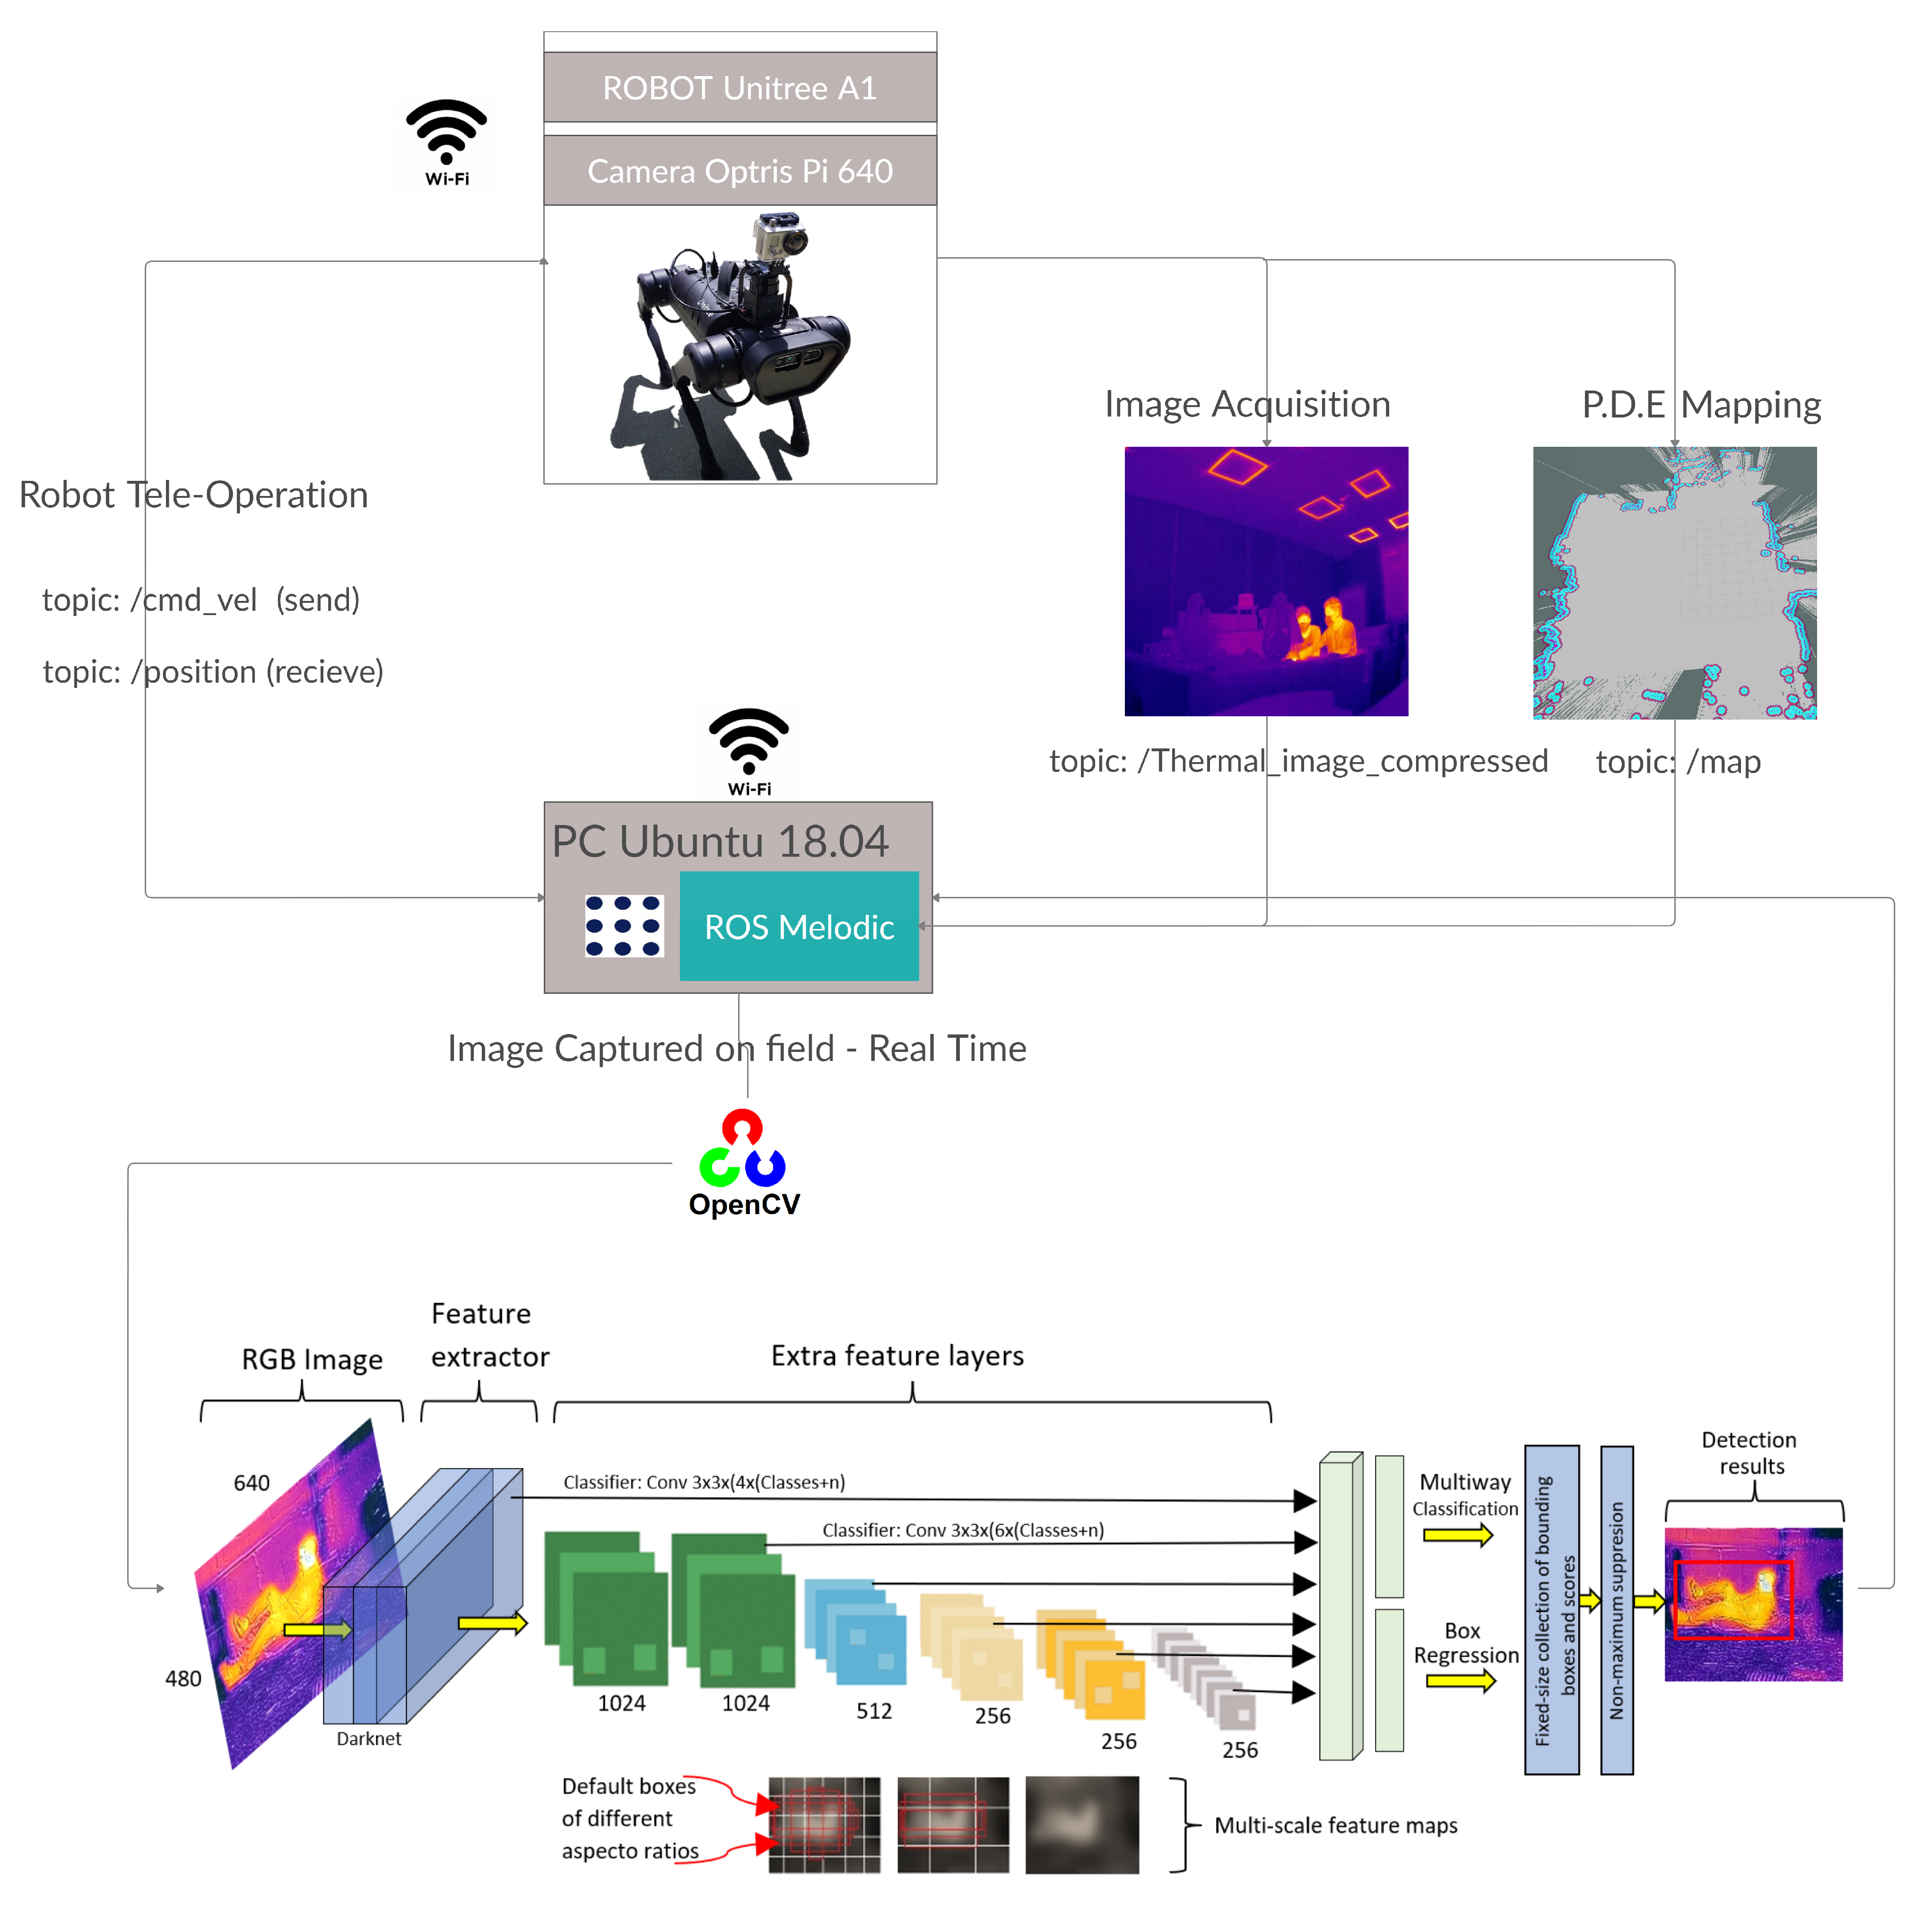
\includegraphics[scale=0.065]{gambar/unitreea1.png}
  % Keterangan gamßbar yang diinputkan
  \caption{\emph{Quadruped robot} dengan kamera termal untuk deteksi korban}
  % Label referensi dari gambar yang diinputkan
  \label{fig:Quadruped  dengan kamera termal untuk deteksi korban}
\end{figure}


\subsection{\emph{Image Processing Technique Applied to Electrical
Substations Based on Drones With Thermal Vision
for Predictive Maintenance}}
Penelitian ini mengusulkan penggunaan \emph{VANT} (Vehículo Aéreo No Tripulado) atau drone, yang dilengkapi dengan dua jenis kamera: \emph{kamera tradisional} untuk menangkap gambar visual dan \emph{kamera termografik} untuk memperoleh gambar inframerah yang dapat menunjukkan suhu komponen di gardu induk. Drone ini dilengkapi dengan sistem navigasi dan pengendalian yang memungkinkan operasi otonom di sekitar gardu induk. Data gambar yang diambil oleh drone diproses menggunakan teknik \emph{image processing} untuk mengidentifikasi \emph{hot spots} atau titik panas pada komponen gardu induk. Hasil analisis ini dapat digunakan untuk memprediksi potensi kerusakan pada komponen dan mengambil tindakan pencegahan yang diperlukan. Penelitian ini menunjukkan bahwa penggunaan drone dengan kamera termal dapat meningkatkan efisiensi dan akurasi dalam pemantauan gardu induk, serta meminimalkan risiko keselamatan bagi petugas yang harus melakukan inspeksi langsung di lokasi gardu \cite{Prieto2022}. Penelitian ini memiliki kesamaan dengan topik kami yang juga menggunakan kamera termal untuk pemantauan komponen gardu listrik.

\begin{figure} [H] \centering
  % Nama dari file gambar yang diinputkan
  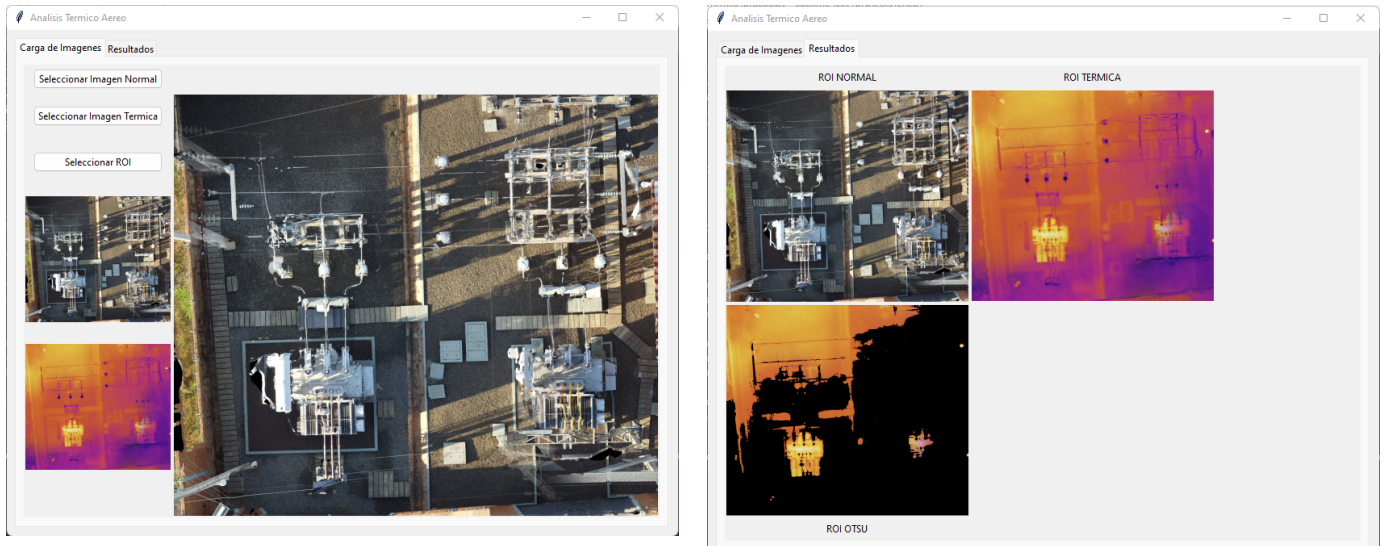
\includegraphics[scale=0.6]{gambar/drone.png}
  % Keterangan gamßbar yang diinputkan
  \caption{Drone dengan kamera termal untuk pemantauan gardu induk}
  % Label referensi dari gambar yang diinputkan
  \label{fig:Drone dengan kamera termal untuk pemantauan gardu induk}
\end{figure}

\subsection{\emph{Direct LiDAR Odometry: Fast Localization With
Dense Point Clouds}}
Penelitian ini berfokus pada pengembangan \emph{Direct LiDAR Odometry} (DLO), sebuah solusi odometri berbasis LiDAR yang \emph{ringan} dan \emph{efisien} untuk robot otonom yang bekerja di lingkungan tanpa sinyal GPS. Sistem ini mengelola informasi peta historis secara efisien dengan cara menyimpan data yang relevan dan mengurangi beban komputasi. DLO memungkinkan penggunaan kembali informasi peta sebelumnya tanpa mengorbankan \emph{kecepatan} dan \emph{akurasi}. DLO menggunakan solver iteratif yang cepat dalam mencocokkan data titik LiDAR, memungkinkan pendaftaran data yang lebih efisien. Teknik ini dipadukan dengan penggunaan kembali struktur data, yang mengurangi waktu pemrosesan dan meningkatkan efisiensi. Sebagai hasilnya, DLO lebih \emph{akurat} dalam menentukan posisi robot dibandingkan dengan metode LiDAR odometry yang ada.

Selain itu, DLO memiliki \emph{beban komputasi yang lebih rendah}, menjadikannya lebih cocok untuk platform robot yang memiliki keterbatasan dalam sumber daya komputasi. Metode ini telah diuji secara ekstensif dalam berbagai lingkungan menantang pada robot udara dan berkaki, termasuk dalam konteks penelitian tim NASA JPL CoSTAR untuk \emph{DARPA Subterranean Challenge} \cite{Chen2022}. Penelitian ini memiliki keterkaitan dengan sistem yang sedang dikembangkan, yang menawarkan sistem lokalisasi tanpa hanya menggunakan GPS, namun tetap \emph{akurat} dan \emph{ringan}. Sistem ini juga diimplementasikan pada robot berkaki (\emph{quadrupped robot}), dengan tujuan untuk memberikan solusi navigasi yang efisien dalam lingkungan yang memiliki medan yang tidak rata dan tidak memiliki sinyal GPS yang memadai.

\begin{figure} [H] \centering
  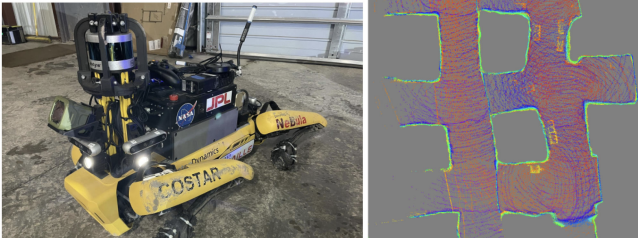
\includegraphics{gambar/dlo.png}
  \caption{Implementasi \emph{DLO} pada \emph{quadruped ledggged robot Boston Dynamics Spot}}
  \label{fig:Implementasi DLO pada quadruped legged robot Boston Dynamics Spot}
\end{figure}

\section{Teori/Konsep Dasar}
Bagian ini berisi pembahasan mengenai teori-teori dasar yang digunakan dalam tugas akhir. Pada bab ini akan dijelaskan mengenai teori-teori yang digunakan dalam penelitian ini. 

\subsection{Gardu listrik}
Gardu listrik merupakan fasilitas yang berfungsi sebagai titik penghubung antara pembangkit listrik dan jaringan distribusi. Gardu berperan penting dalam mengatur dan mendistribusikan tenaga listrik ke konsumen akhir. Terdapat berberapa jenis gardu listrik beberapa diantaranya adalah gardu induk dan gardu pembangkit. Gardu induk adalah fasilitas yang berfungsi untuk mengubah tegangan tinggi menjadi tegangan rendah, sehingga dapat didistribusikan ke konsumen dengan aman. Di sisi lain, gardu pembangkit adalah fasilitas yang terletak di dekat sumber energi, seperti pembangkit listrik tenaga air atau pembangkit listrik tenaga uap, yang berfungsi untuk mengubah energi dari sumber tersebut menjadi energi listrik dan mendistribusikannya ke jaringan listrik. Gardu dilengkapi dengan berbagai peralatan, seperti transformator, pemutus sirkuit, dan isolator, yang berfungsi untuk menjaga kestabilan dan keandalan pasokan listrik. 

\subsubsection{Transformator}
Transformator merupakan komponen esensial dalam sistem kelistrikan, yang berfungsi untuk mengubah tegangan listrik serta memastikan distribusi energi berlangsung secara efisien.

\begin{figure} [H] \centering
  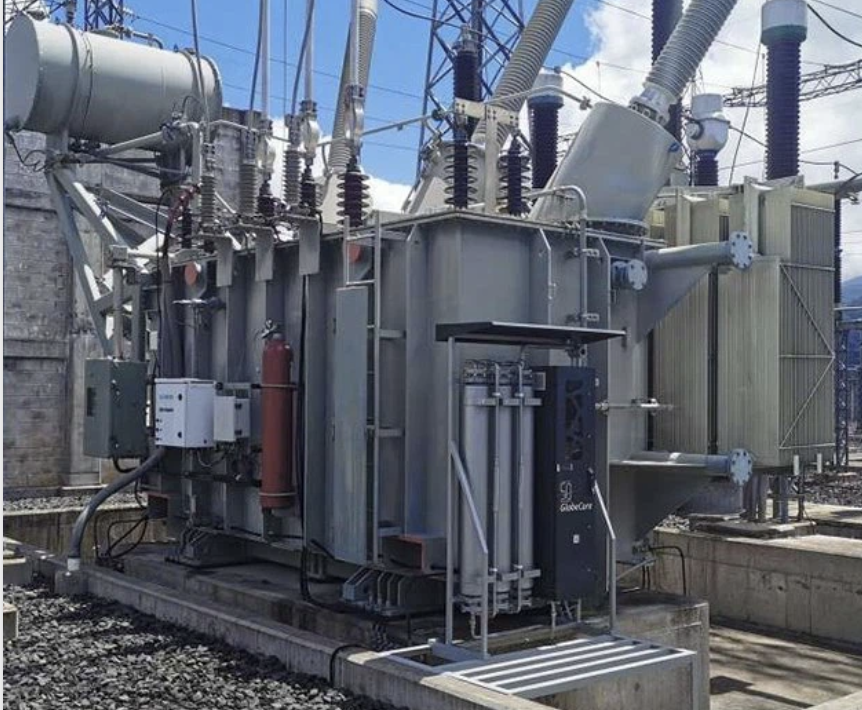
\includegraphics[scale=0.45]{gambar/trafo.png}
  \caption{Transformator gardu listrik}
  \label{fig:Transformator gardu listrik}
\end{figure}

Prinsip kerja transformator ini didasarkan pada induksi elektromagnetik, yaitu mengubah tegangan listrik dari tinggi ke rendah atau sebaliknya, sesuai dengan kebutuhan sistem distribusi. Secara umum, transformator gardu induk terdiri dari dua bagian utama, yaitu bagian inti besi dan gulungan kumparan. Selain itu, transformator ini juga dilengkapi dengan komponen-komponen penting seperti \emph{bushing}, \emph{tap changer}, dan \emph{cooling system}, yang berperan penting dalam menjaga kinerja serta keandalan transformator. Suhu operasi normal transformator umumnya berkisar antara 40\textdegree{}C hingga 80\textdegree{}C, tergantung pada kapasitas dan spesifikasi teknis transformator tersebut.\cite{tambunan2023kerja}.

\subsubsection{Arester}
\emph{Arester}, atau \emph{lightning arrester}, adalah perangkat yang melindungi sistem kelistrikan dari lonjakan tegangan akibat petir. \emph{Arester} berfungsi untuk mengalihkan arus petir ke tanah, sehingga melindungi peralatan listrik dari kerusakan. 

\begin{figure} [H] \centering
  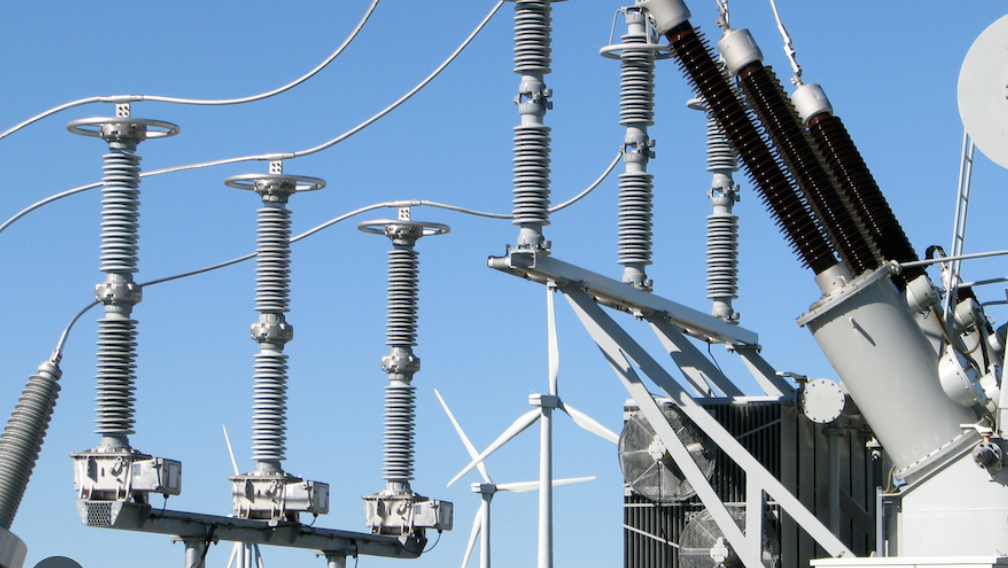
\includegraphics[scale=0.45]{gambar/arestar.png}
  \caption{Arester gardu listrik}
  \label{fig:Arester gardu listrik}
\end{figure}

Penelitian menunjukkan bahwa untuk memastikan efektivitas \emph{arester}, nilai resistansi pembumian harus rendah, idealnya di bawah 10 $\Omega$. Selain itu, pemeliharaan rutin terhadap \emph{arester} sangat penting untuk memastikan kinerjanya tetap optimal, termasuk pengujian terhadap kondisi lingkungan yang dapat mempengaruhi performanya \cite{Suputra2024}. Suhu operasi \emph{arester} biasanya berkisar antara -40°C hingga 60°C. Suhu melebihi batas maksimum dapat menyebabkan kerusakan permanen pada perangkat tersebut \cite{Kartika2022}.

\subsubsection{Disconnector}
\emph{Disconnector}, atau pemisah, adalah perangkat yang digunakan untuk memutuskan arus listrik dalam sistem distribusi. 
\begin{figure} [H] \centering
  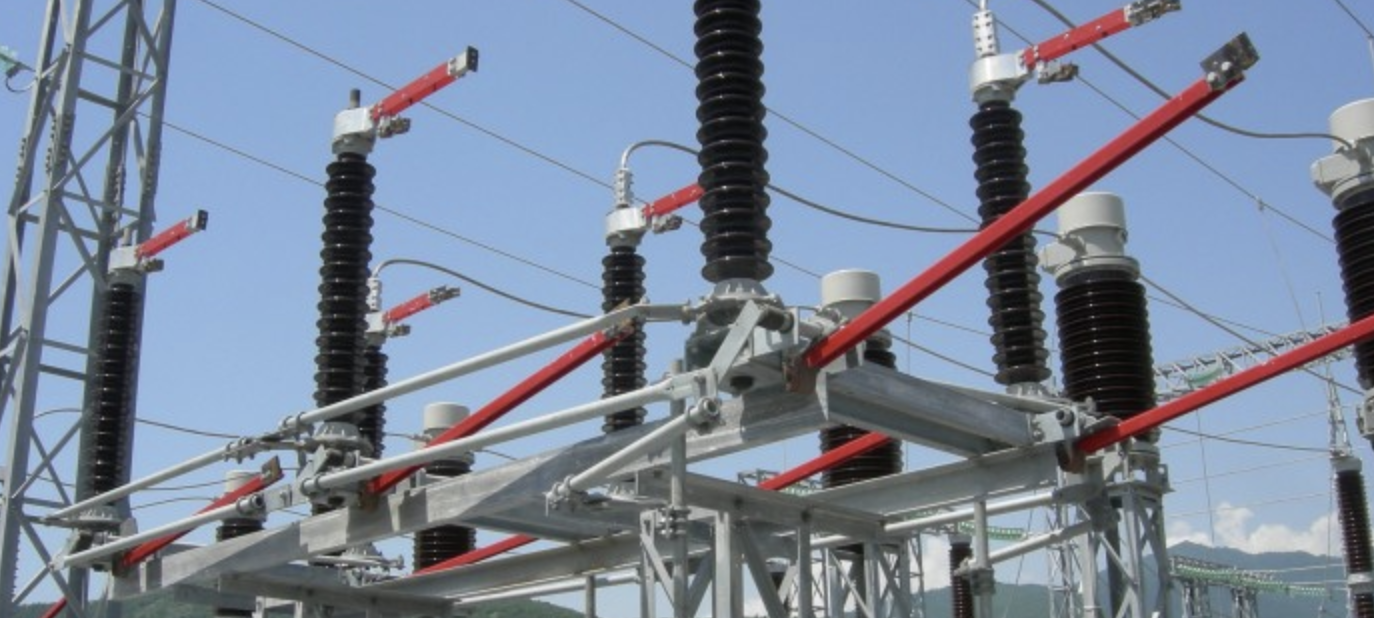
\includegraphics[scale=0.45]{gambar/disconector.png}
  \caption{Disconnector gardu listrik}
  \label{fig:Disconnector gardu listrik}
\end{figure}

\emph{Disconnector} berfungsi untuk memisahkan bagian dari sistem kelistrikan untuk keperluan pemeliharaan atau perbaikan tanpa mempengaruhi bagian lain dari jaringan. Pemeliharaan dan pengujian berkala terhadap \emph{disconnector} sangat penting untuk memastikan bahwa perangkat ini berfungsi dengan baik saat dibutuhkan. Suhu operasi \emph{disconnector} biasanya berada dalam rentang 20°C hingga 40°C, dan overheating dapat terjadi jika suhu melebihi 85°C, yang dapat mengakibatkan kegagalan fungsi\cite{Henriana2022}.

\subsubsection{Busbar}
\emph{Busbar} adalah komponen penting dalam gardu listrik yang berfungsi sebagai penghubung antara berbagai peralatan listrik. \emph{Busbar} memungkinkan distribusi arus listrik yang efisien dan aman di dalam gardu. \emph{Busbar} biasanya terbuat dari bahan konduktif yang baik, seperti tembaga atau aluminium, dan dirancang untuk menampung arus listrik dalam jumlah besar. Pemeliharaan dan pengujian \emph{busbar} secara rutin diperlukan untuk mencegah kerusakan dan memastikan keandalan sistem distribusi listrik. Suhu operasi \emph{busbar} dapat bervariasi, tetapi umumnya tidak boleh melebihi 90°C untuk mencegah overheating yang dapat merusak isolasi dan struktur busbar itu sendiri \cite{Telaumbanua2024}.

\subsubsection{Isolator}
\emph{Isolator} adalah perangkat yang berfungsi untuk memisahkan bagian dari sistem kelistrikan, sehingga mencegah arus listrik mengalir ke bagian yang tidak diinginkan. \emph{Isolator} digunakan untuk menjaga keamanan dan keandalan sistem kelistrikan, terutama saat pemeliharaan dilakukan. \emph{Isolator} dirancang untuk menahan tegangan tinggi dan memiliki karakteristik dielektrik yang baik. Pemeliharaan \emph{isolator} juga penting untuk memastikan bahwa tidak ada kebocoran arus yang dapat menyebabkan kerusakan pada peralatan lainnya. Suhu operasi \emph{isolator} biasanya berkisar antara -30°C hingga 50°C, dan overheating dapat terjadi jika suhu melebihi 70°C, yang dapat mengakibatkan kerusakan pada material isolasi \cite{Moreno2017}.

\subsubsection{Pemutus Sirkuit (\emph{Circuit Breaker})}

\emph{Pemutus sirkuit} adalah perangkat yang berfungsi untuk melindungi sistem kelistrikan dari arus lebih (\emph{overcurrent}) dan hubung singkat (\emph{short circuit}). \emph{Pemutus sirkuit} dapat secara otomatis memutuskan aliran listrik ketika terdeteksi adanya gangguan, sehingga mencegah kerusakan pada peralatan dan menjaga keselamatan sistem. Terdapat berbagai jenis \emph{pemutus sirkuit}, termasuk \emph{pemutus sirkuit otomatis} (\emph{automatic circuit breaker}) dan \emph{pemutus sirkuit manual} (\emph{manual circuit breaker}), yang masing-masing memiliki aplikasi dan karakteristik yang berbeda. 

\begin{figure} [H] \centering
  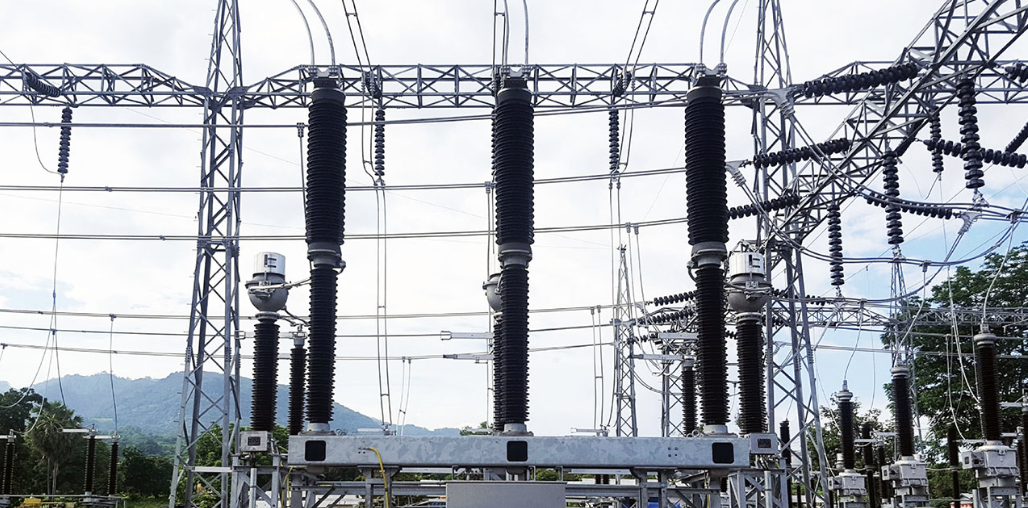
\includegraphics[scale=0.45]{gambar/cb.png}
  \caption{Pemutus sirkuit gardu listrik}
  \label{fig:cb gardu listrik}
\end{figure}
Pemeliharaan dan pengujian berkala terhadap \emph{pemutus sirkuit} sangat penting untuk memastikan bahwa perangkat ini berfungsi dengan baik saat dibutuhkan. Suhu operasi \emph{pemutus sirkuit} biasanya berkisar antara -25°C hingga 55°C, dan overheating dapat terjadi jika suhu melebihi 85°C, yang dapat menyebabkan kerusakan pada mekanisme pemutus \cite{Ilomets2020}.


\subsection{\emph{DeepRobotics Jueying Lite 3 Quadruped Robot}}
DeepRobotics Jueying Lite 3 adalah robot \emph{quadruped} yang dikembangkan oleh DeepRobotics, sebuah perusahaan teknologi robotik di China. Robot ini dirancang untuk berbagai aplikasi, termasuk eksplorasi, pemantauan, dan layanan di berbagai lingkungan. Dengan desain yang ringkas dan kuat, \emph{Jueying Lite 3} mampu bergerak dengan cepat dan stabil di medan yang beragam, menjadikannya ideal untuk aplikasi di luar ruangan. Untuk menjaga stabilitas, \emph{Jueying Lite 3} menerapkan model \emph{3D-SLIP (Three-Dimensional Spring-Loaded Inverted Pendulum)} yang dirancang untuk menjaga keseimbangan saat robot bergerak di medan tidak rata.\cite{deep2024perception}.

\emph{Jueying Lite 3} dilengkapi dengan \emph{neural network} yang telah dilatih sebelumnya untuk meningkatkan kinerja gerakan \emph{bounding} dan kontrol umpan balik. Dengan fungsi penghargaan yang mempertimbangkan titik kontak dan fase gerakan, robot mencapai simetri dan periodisitas gerakan yang lebih baik, sehingga meningkatkan efisiensi mobilitas. Estimasi keadaan robot dilakukan melalui metode \emph{Extended Kalman Filter} (EKF) yang dimodifikasi, yang meningkatkan akurasi estimasi di medan tidak stabil, memungkinkan robot mengatasi slip pada kaki dan beradaptasi terhadap berbagai jenis medan. Selain itu untuk kontrol eksternal, \emph{Jueying Lite 3} dapat dikendalikan melalui \emph{ROS URI} dengan mengirimkan topik \texttt{cmd\_vel}\cite{deep2024motion}.

\subsection{\emph{Robot Operating System (ROS)}}
\emph{Robot Operating System (ROS)} adalah \emph{framework} perangkat lunak \emph{open-source} yang dirancang untuk memfasilitasi pengembangan aplikasi robotik. ROS menyediakan berbagai \emph{tools} dan \emph{libraries} untuk mengelola berbagai tugas robotik, seperti kontrol aktuator, pemrosesan data sensor, serta navigasi dan kontrol gerak. Salah satu keunggulan ROS adalah arsitekturnya yang modular, memungkinkan pengembang untuk membagi sistem robotik kompleks menjadi bagian-bagian kecil yang saling terhubung, dikenal sebagai \emph{node}. ROS mendukung berbagai aplikasi robotik, mulai dari robot industri hingga robot otonom. Berikut adalah beberapa komponen dan konsep penting dalam ROS:

\subsubsection{\emph{Node}}
\emph{Node} adalah unit dasar dalam ROS yang berfungsi sebagai proses independen untuk menjalankan tugas spesifik dalam sistem robotik. Setiap \emph{node} memiliki fungsionalitas tertentu, seperti mengambil data sensor atau mengontrol aktuator, dan dapat berkomunikasi dengan \emph{node} lainnya melalui berbagai mekanisme komunikasi, seperti \emph{topic}, \emph{service}, atau \emph{action}. \emph{Node} bekerja secara paralel dan saling berinteraksi untuk membentuk aplikasi robotik yang kompleks.

\subsubsection{\emph{Topic}}
\emph{Topic} adalah mekanisme komunikasi \emph{publish/subscribe} antara \emph{node} untuk pertukaran data secara asinkron. \emph{Node} yang berfungsi sebagai \emph{publisher} mengirimkan data ke \emph{topic}, sementara \emph{node} yang berfungsi sebagai \emph{subscriber} menerima data dari \emph{topic} tersebut. Data yang dikirim melalui \emph{topic} biasanya berbentuk pesan (\emph{message}) yang memiliki format tertentu yang disepakati oleh pengembang.

\subsubsection{\emph{Service}}
\emph{Service} adalah mekanisme komunikasi sinkron antara dua \emph{node}, di mana satu \emph{node} melakukan permintaan (\emph{request}) dan \emph{node} lainnya memberikan respon (\emph{response}) secara langsung. Layanan ini berguna untuk tugas-tugas yang memerlukan hasil segera setelah permintaan dilakukan, seperti pengaturan parameter robot atau pembacaan nilai sensor tertentu.

\subsubsection{\emph{Action}}
\emph{Action} digunakan untuk tugas-tugas yang memerlukan umpan balik berkelanjutan dan memungkinkan komunikasi dua arah antara \emph{node}. Berbeda dengan \emph{service}, yang bersifat sinkron dan langsung, \emph{action} mendukung komunikasi asinkron dengan menyediakan umpan balik selama operasi berlangsung, seperti pada tugas pergerakan robot yang memerlukan estimasi waktu dan status secara dinamis.

\subsubsection{\emph{Launch File}}
\emph{Launch File} adalah file berformat XML yang digunakan untuk menginisiasi beberapa \emph{node} dan parameter konfigurasi secara bersamaan. \emph{Launch file} memungkinkan pengembang untuk menyusun dan mengelola konfigurasi sistem robotik dengan lebih efisien, menghindari pengaturan manual yang berulang kali. File ini dapat digunakan untuk menentukan urutan \emph{node} yang dijalankan serta parameter yang diperlukan.

\subsubsection{\emph{Bag File}}
\emph{Bag File} adalah format file yang digunakan untuk merekam dan memutar ulang data \emph{topic}. \emph{Bag file} sangat berguna dalam pengujian dan debugging karena memungkinkan pengembang untuk memeriksa data yang dikumpulkan sebelumnya tanpa perlu menjalankan robot secara langsung. Dengan menggunakan \emph{bag file}, data dapat diputar ulang untuk melakukan analisis atau pengujian lebih lanjut.

\subsubsection{\emph{Package}}
\emph{Package} adalah unit dasar dalam ROS yang mengorganisir \emph{node}, \emph{libraries}, dan file konfigurasi yang diperlukan oleh aplikasi robotik. Setiap paket dapat berisi kode sumber, file eksekusi, dan file konfigurasi yang mendukung tugas tertentu dalam sistem robot. Paket memungkinkan pengelolaan dan pemeliharaan proyek robotik menjadi lebih terstruktur dan modular.

\subsubsection{\emph{Parameter}}
\emph{Parameter} adalah variabel dinamis yang disimpan dalam server parameter ROS. \emph{Parameter} ini memungkinkan \emph{node} untuk berbagi informasi konfigurasi secara global dalam sistem. Dengan menggunakan \emph{parameter}, pengembang dapat mengubah konfigurasi robot secara lebih fleksibel tanpa perlu mengubah kode sumber. \emph{Parameter} biasanya digunakan untuk menyimpan nilai-nilai yang digunakan oleh beberapa \emph{node}, seperti kecepatan robot atau batasan sensor.

\subsubsection{\emph{Workspace}}
\emph{Workspace} adalah direktori kerja dalam ROS tempat pengembang mengelola \emph{package}, \emph{build}, dan konfigurasi pengembangan. \emph{Workspace} umumnya terdiri dari folder seperti \texttt{src} untuk menyimpan kode sumber, \texttt{devel} untuk hasil \emph{build}, dan \texttt{install} untuk menampung hasil instalasi. Dengan menggunakan \emph{workspace}, pengembang dapat mengelola proyek ROS secara terstruktur dan efisien.

\subsubsection{\emph{tf}}
\emph{tf} adalah sebuah paket dalam ROS yang digunakan untuk melacak hubungan koordinat antara berbagai frame dalam sistem robotik. \emph{tf} memungkinkan pengembang untuk melakukan transformasi antara berbagai frame koordinat (misalnya, frame robot dan frame dunia) secara efisien, sehingga koordinat objek dan sensor dapat diubah sesuai dengan referensi yang dibutuhkan. Misalnya, dalam robot otonom, \emph{tf} digunakan untuk mengetahui posisi dan orientasi robot dalam peta atau untuk menghitung posisi objek yang terdeteksi oleh sensor.

Dengan menggunakan \emph{tf}, pengembang dapat menghindari kesalahan dalam kalkulasi posisi dan orientasi, yang sangat penting dalam aplikasi robotik yang melibatkan navigasi dan interaksi dengan lingkungan. Paket \emph{tf} menyediakan berbagai fungsi untuk mengatur dan mengelola transformasi koordinat, seperti \texttt{tf::TransformListener} yang digunakan untuk mendengarkan perubahan transformasi, dan \texttt{tf::TransformBroadcaster} untuk mempublikasikan transformasi koordinat \cite{ros_noetic}.

\subsection{\emph{Kamera Termal}}
Kamera termal adalah perangkat yang digunakan untuk mendeteksi distribusi suhu secara non-kontak melalui radiasi inframerah yang dipancarkan oleh objek. Setiap objek dengan suhu di atas nol absolut memancarkan radiasi inframerah, dan kamera termal mengonversi radiasi tersebut menjadi gambar yang menampilkan variasi suhu dalam bentuk skala warna. Citra termal memvisualisasikan suhu dengan menggunakan skala warna, di mana warna biru dan ungu menandakan suhu rendah, hijau dan kuning menunjukkan suhu sedang, serta merah dan putih menunjukkan suhu tinggi atau overheat, seperti yang ditunjukkan pada gambar \ref{fig:thermal diagram}.


\begin{figure} [H] \centering
  % Nama dari file gambar yang diinputkan
  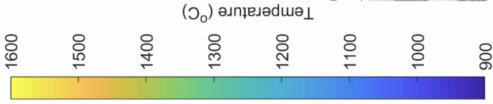
\includegraphics[scale=0.45]{gambar/thermal_range.png}
  % Keterangan gambar yang diinputkan
  \caption{Suhu berdasrakan warna pada kamera thermal}
  % Label referensi dari gambar yang diinputkan
  \label{fig:thermal diagram}
\end{figure}


Penggunaan skala warna ini memudahkan interpretasi visual, terutama dalam aplikasi industri, seperti pemantauan transformator untuk mendeteksi overheating yang dapat menyebabkan kegagalan operasional. Selain itu, kamera termal banyak digunakan dalam pemantauan industri untuk mendeteksi panas berlebih pada peralatan listrik, serta dalam bidang medis dan konstruksi untuk deteksi masalah suhu atau kelembaban\cite{kartono2023pemanfaatan}.

\subsection{\emph{Computer Vision}}
\emph{Computer vision} merupakan cabang dari kecerdasan buatan yang memungkinkan komputer memahami dan menganalisis informasi yang diperoleh dari gambar atau video digital. Berbeda dengan manusia yang secara alami "belajar" untuk menginterpretasikan konteks, jarak objek, serta mendeteksi apakah objek tersebut bergerak atau diam, \emph{computer vision} membutuhkan pemrograman yang kompleks untuk meniru kemampuan tersebut. Salah satu kemajuan terbesar dalam bidang \emph{computer vision} adalah pengembangan arsitektur \emph{Convolutional Neural Network} (CNN), yang menjadi dasar untuk berbagai aplikasi seperti klasifikasi citra, segmentasi, hingga deteksi objek. Salah satu algoritma yang dibangun berdasarkan \emph{CNN} adalah YOLOv8. YOLOv8 (You Only Look Once versi 8) merupakan algoritma deteksi objek yang terkenal dengan efisiensinya dalam melakukan deteksi objek secara real-time. Algoritma ini dirancang untuk mendeteksi objek hanya dengan satu kali melihat gambar secara menyeluruh, tanpa perlu membaginya menjadi beberapa bagian, yang menjadikannya lebih cepat dibandingkan metode deteksi objek lainnya.

YOLOv8 membawa sejumlah peningkatan signifikan dibandingkan pendahulunya, seperti optimasi dalam deteksi multi-skala, yang memungkinkan algoritma ini mengenali objek dengan berbagai ukuran dalam satu citra. Selain itu, YOLOv8 juga dilengkapi dengan model yang lebih ringan dan efisien, sehingga dapat diterapkan pada perangkat dengan kemampuan komputasi terbatas. Model ini juga menggunakan \emph{backbone} yang lebih efisien dan \emph{neck} yang ditingkatkan untuk meningkatkan ekstraksi fitur, memungkinkan deteksi yang lebih akurat dan cepat pada berbagai jenis objek dan skenario aplikasi. Dengan kemampuan \emph{deep learning} yang lebih maju, YOLOv8 tidak hanya mampu mendeteksi objek secara cepat, tetapi juga memberikan hasil yang lebih akurat. Hal ini membuatnya sangat cocok untuk berbagai aplikasi yang membutuhkan deteksi objek real-time, seperti sistem pemantauan, kendaraan otonom, dan pemrosesan video untuk keamanan \cite{yolov8}.


\subsection{Metode Evaluasi dalam \emph{Computer Vision}}
Dalam bidang \emph{computer vision}, evaluasi kinerja model sangat penting untuk menilai kemampuan sistem dalam mengidentifikasi dan mengklasifikasikan objek. Beberapa metrik yang sering digunakan untuk mengevaluasi performa model \emph{computer vision} antara lain adalah \emph{confusion matrix}, \emph{precision}, \emph{recall}, \emph{accuracy}, \emph{F1 score}, dan \emph{loss function}. Metrik-metrik ini memberikan informasi yang lebih mendalam mengenai kinerja model selain hanya menggunakan tingkat akurasi.

\subsubsection{\emph{Confusion Matrix}}
\emph{Confusion matrix} adalah tabel yang digunakan untuk mendeskripsikan kinerja model klasifikasi. Matriks ini mencatat jumlah prediksi yang benar dan salah, baik dalam kategori positif maupun negatif. Sebuah matriks konfusi untuk klasifikasi biner dapat digambarkan sebagai berikut:

\begin{figure} [H] \centering
  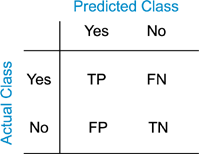
\includegraphics[scale=0.7]{gambar/cf.png}
  \caption{Contoh \emph{confusion matrix} untuk klasifikasi biner}
  \label{fig:cf}
\end{figure}

\subsubsection{\emph{Precision}, \emph{Recall}, dan \emph{Accuracy}}
\emph{Precision} dan \emph{recall} adalah dua metrik penting dalam evaluasi model klasifikasi. \emph{Precision} mengukur seberapa akurat prediksi positif yang dilakukan oleh model, sedangkan \emph{recall} mengukur seberapa banyak contoh positif yang berhasil ditemukan oleh model.

\emph{Precision} dihitung sebagai:

\begin{equation}
  Precision = \frac{TP}{TP + FP}
\end{equation}

\emph{Recall} dihitung sebagai:

\begin{equation}
 Recall = \frac{TP}{TP + FN}
\end{equation}

\emph{Accuracy} mengukur seberapa banyak prediksi yang benar dilakukan oleh model, dan dihitung sebagai:

\begin{equation}
 Accuracy = \frac{TP + TN}{TP + TN + FP + FN}
\end{equation}

\subsubsection{\emph{F1 Score}}
\emph{F1 score} adalah metrik yang merupakan rata-rata harmonis dari \emph{precision} dan \emph{recall}. Metrik ini memberikan gambaran yang lebih seimbang mengenai kinerja model, terutama ketika terdapat ketidakseimbangan antara kelas-kelas dalam data.

\emph{F1 score} dihitung sebagai:

\begin{equation}
  F_1 = 2 \times \frac{P \times R}{P + R}.
\end{equation}


\subsubsection{\emph{Loss Function}}
\emph{Loss function} adalah metrik yang digunakan untuk menghitung seberapa jauh prediksi model dari nilai yang sebenarnya. Dalam \emph{computer vision}, loss function sangat penting untuk mengoptimalkan model selama pelatihan. Salah satu loss function yang umum digunakan dalam masalah klasifikasi adalah \emph{cross-entropy loss}, yang menghitung perbedaan antara distribusi probabilitas yang diprediksi dan distribusi probabilitas yang sebenarnya.

Dalam klasifikasi multi-kelas, \emph{cross-entropy loss} dihitung sebagai:

\begin{equation}
L = -\sum_{i=1}^{C} y_i \log(p_i)
\end{equation}

Di mana \( C \) adalah jumlah kelas, \( y_i \) adalah label asli untuk kelas ke-i, dan \( p_i \) adalah probabilitas yang diprediksi untuk kelas ke-i.


\subsubsection{IMU dan Odometry Fusion dengan \textit{Extended Kalman Filter} (EKF)}
Pada tahap prediksi, model dinamik digunakan untuk memprediksi keadaan berdasarkan kontrol yang diterima. Misalkan vektor keadaan \( \hat{x}_{k|k-1} \) pada waktu \( k-1 \) dan kontrol \( u_{k-1} \):

\begin{equation}
\hat{x}_{k|k-1} = f(\hat{x}_{k-1}, u_{k-1})
\end{equation}

Di mana \( f(\hat{x}_{k-1}, u_{k-1}) \) adalah fungsi non-linear yang menggambarkan evolusi keadaan sistem. Pengukuran dari IMU dan odometry digunakan untuk memperbarui estimasi keadaan. Kalman gain dihitung dengan:

\begin{equation}
K_k = P_{k|k-1} H_k^T \left( H_k P_{k|k-1} H_k^T + R_k \right)^{-1}
\end{equation}

Estimasi posisi dan orientasi diperbarui dengan:

\begin{equation}
\hat{x}_k = \hat{x}_{k|k-1} + K_k \left( z_k - h(\hat{x}_{k|k-1}) \right)
\end{equation}

Kovarians pembaruan dihitung dengan:

\begin{equation}
P_k = (I - K_k H_k) P_{k|k-1}
\end{equation}

Fusion data IMU dan odometry dengan EKF meningkatkan akurasi estimasi posisi dan orientasi dengan mengurangi ketidakpastian pada masing-masing sumber data \cite{barbosa2016}.


\subsection{PID Controller}
PID controller merupakan salah satu metode kontrol yang paling sering digunakan dalam berbagai aplikasi, karena memiliki struktur yang sederhana dengan hanya tiga parameter utama. Hal tersebut membuat PID controller lebih mudah dioperasikan dan dipahami oleh teknisi dibandingkan dengan metode kontrol lain yang lebih kompleks. PID controller terdiri dari tiga komponen utama, yaitu aksi \emph{proportional}, \emph{integral}, dan \emph{derivative}. Ketiga komponen ini saling melengkapi dalam memperbaiki \emph{error} pada sistem kontrol. \emph{Proportional} memberikan koreksi berdasarkan \emph{error} saat ini, aksi \emph{integral} memperhitungkan \emph{error} masa lalu untuk mengeliminasi offset, dan aksi \emph{derivative} memperkirakan \emph{trend error} untuk respons prediktif. 

\begin{equation}
    u(t) = u_P(t) + u_I(t) + u_D(t) = K_p e(t) + K_i \int_{0}^{t} e(\tau) d\tau + K_d \frac{d}{dt}e(t),
\end{equation}

di mana $K_p$, $K_i$, dan $K_d$ adalah koefisien \emph{gain} yang terkait dengan aksi \emph{proportional}, \emph{integral}, dan \emph{derivative} masing-masing.

\subsection{\emph{Direct LiDAR-Inertial Odometry (DLIO)}}
Algoritma \emph{Direct LiDAR-Inertial Odometry} (DLIO) menawarkan solusi dengan pendekatan \emph{coarse-to-fine} untuk menghasilkan koreksi gerakan waktu kontinu secara lebih akurat. DLIO memanfaatkan persamaan analitik yang dirancang untuk memperbaiki setiap titik data secara paralel dan efisien, sekaligus mengintegrasikan data LiDAR dan \emph{Inertial Measurement Unit} (IMU) secara ketat untuk menghasilkan estimasi keadaan robot yang lebih akurat. Pendekatan ini memungkinkan koreksi distorsi pada \emph{point cloud} secara \emph{real-time}, bahkan dalam kondisi pergerakan dinamis yang kompleks \cite{chen2022dlio}.


\begin{figure} [H] \centering
  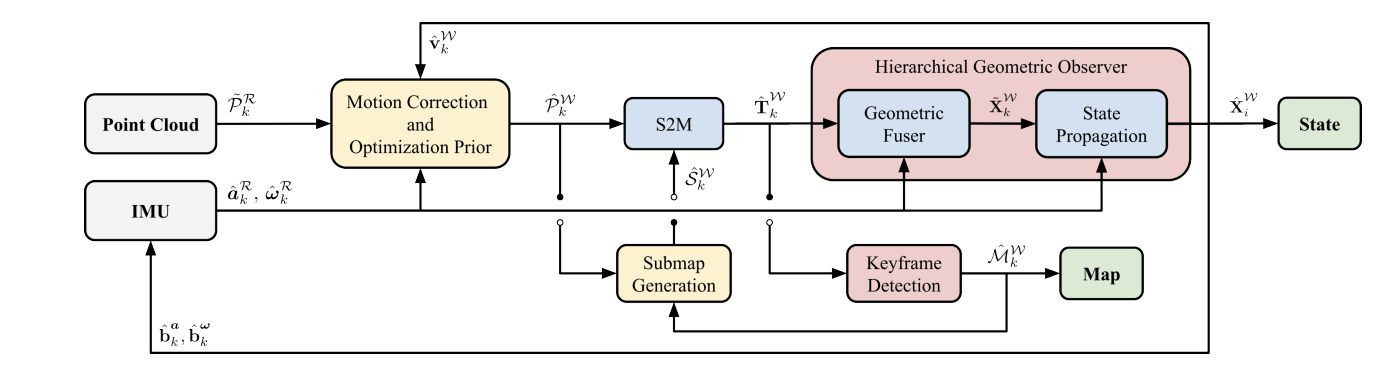
\includegraphics[scale=0.6]{gambar/dlio_Arch.png}
  \caption{Arsitektur \emph{Direct LiDAR-Inertial Odometry (DLIO)}}
  \label{fig:DLIO Architecture}
\end{figure}

Keunggulan DLIO tidak hanya terletak pada akurasi tinggi dalam estimasi posisi, tetapi juga pada efisiensi komputasi yang lebih baik dibandingkan algoritma-algoritma terkini lainnya seperti LIO-SAM dan FAST-LIO2. DLIO menggabungkan koreksi gerakan dan pembuatan \emph{prior} dalam satu langkah, menghilangkan kebutuhan akan \emph{scan-to-scan matching} yang biasanya memakan waktu. Melalui eksperimen pada \emph{dataset} publik dan \emph{dataset} lapangan yang dikumpulkan secara mandiri, DLIO menunjukkan keunggulan dalam menghasilkan peta 3D yang detail dengan kesalahan posisi minimum. Sistem ini menjadi alternatif yang menjanjikan untuk platform robot bergerak, termasuk drone, dalam navigasi dan pemetaan di lingkungan yang tidak terstruktur.

\subsection{WebSocket}
WebSocket adalah protokol komunikasi dua arah yang beroperasi di atas koneksi TCP yang persisten, memungkinkan pertukaran pesan antara klien dan server secara efisien. Protokol ini dirancang untuk mengatasi kekurangan teknologi komunikasi dua arah yang ada sebelumnya, yang sering menggunakan \emph{HTTP} sebagai lapisan transportasi. Dengan memanfaatkan mekanisme \emph{upgrade} dari \emph{HTTP}, WebSocket dapat membuka saluran komunikasi bidirectional yang lebih efisien dibandingkan dengan pendekatan tradisional seperti \emph{polling} atau \emph{long polling} \cite{Fette2011}.

Keunggulan utama dari WebSocket terletak pada kemampuannya untuk mengurangi overhead komunikasi, yang sangat penting dalam aplikasi yang memerlukan pembaruan real-time, seperti aplikasi \emph{chat}, permainan daring, dan sistem \emph{IoT}. Penelitian menunjukkan bahwa WebSocket tidak hanya meningkatkan efisiensi komunikasi, tetapi juga memungkinkan pengembangan aplikasi kolaboratif yang lebih responsif dan interaktif \cite{Milsap2019}. Dengan demikian, WebSocket menjadi solusi yang ideal untuk aplikasi yang membutuhkan latensi rendah dan kecepatan tinggi dalam pertukaran data.
\cleardoublepage

% Bab 3 desain dan implementasi
\chapter{DESAIN DAN IMPLEMENTASI}
\label{chap:desainimplementasi}

% Ubah bagian-bagian berikut dengan isi dari desain dan implementasi

Penelitian ini dilaksanakan sesuai \lipsum[1][1-5]

\section{Deskripsi Sistem}
\label{sec:deskripsisistem}

Sistem akan dibuat dengan \lipsum[1-2]

\section{Implementasi Alat
  \label{sec:implementasi alat}}

Alat diimplementasikan dengan \lipsum[1]

% Contoh pembuatan potongan kode
\begin{lstlisting}[
  language=C++,
  caption={Program halo dunia.},
  label={lst:halodunia}
]
#include <iostream>

int main() {
    std::cout << "Halo Dunia!";
    return 0;
}
\end{lstlisting}

\lipsum[2-3]

% Contoh input potongan kode dari file
\lstinputlisting[
  language=Python,
  caption={Program perhitungan bilangan prima.},
  label={lst:bilanganprima}
]{program/bilangan-prima.py}

\lipsum[4]

\cleardoublepage

% Bab 4 pengujian dan analisis
\chapter{PENGUJIAN DAN ANALISIS}
\label{chap:pengujiananalisis}

% Ubah bagian-bagian berikut dengan isi dari pengujian dan analisis

Pada penelitian ini dipaparkan \lipsum[1][1-5]

\section{Skenario Pengujian}
\label{sec:skenariopengujian}

Pengujian dilakukan dengan \lipsum[1-2]

\section{Evaluasi Pengujian}
\label{sec:analisispengujian}

Dari pengujian yang \lipsum[1]

% Contoh pembuatan tabel
\begin{longtable}{|c|c|c|}
  \caption{Hasil Pengukuran Energi dan Kecepatan}
  \label{tb:EnergiKecepatan}                                   \\
  \hline
  \rowcolor[HTML]{C0C0C0}
  \textbf{Energi} & \textbf{Jarak Tempuh} & \textbf{Kecepatan} \\
  \hline
  10 J            & 1000 M                & 200 M/s            \\
  20 J            & 2000 M                & 400 M/s            \\
  30 J            & 4000 M                & 800 M/s            \\
  40 J            & 8000 M                & 1600 M/s           \\
  \hline
\end{longtable}

\lipsum[2-4]

\cleardoublepage

% Bab 5 penutup
\chapter{PENUTUP}
\label{chap:penutup}

% Ubah bagian-bagian berikut dengan isi dari penutup

\section{Kesimpulan}
\label{sec:kesimpulan}

Berdasarkan hasil pengujian yang \lipsum[1][1-3] sebagai berikut:

\begin{enumerate}[nolistsep]

  \item Pembuatan \lipsum[2][1-3]

  \item \lipsum[2][4-6]

  \item \lipsum[2][7-10]

\end{enumerate}

\section{Saran}
\label{chap:saran}

Untuk pengembangan lebih lanjut pada \lipsum[1][1-3] antara lain:

\begin{enumerate}[nolistsep]

  \item Memperbaiki \lipsum[2][1-3]

  \item \lipsum[2][4-6]

  \item \lipsum[2][7-10]

\end{enumerate}

\cleardoublepage

\chapter*{DAFTAR PUSTAKA}
\addcontentsline{toc}{chapter}{DAFTAR PUSTAKA}
\renewcommand\refname{}
\vspace{2ex}
\renewcommand{\bibname}{}
\begingroup
\def\chapter*#1{}
\printbibliography
\endgroup
\cleardoublepage

% Biografi penulis
\begin{center}
  \Large
  \textbf{BIOGRAFI PENULIS}
\end{center}

\addcontentsline{toc}{chapter}{BIOGRAFI PENULIS}

\vspace{2ex}

\begin{wrapfigure}{L}{0.3\textwidth}
  \centering
  \vspace{-3ex}
  % Ubah file gambar berikut dengan file foto dari mahasiswa
  
\includegraphics[width=0.3\textwidth]{gambar/elon.jpg}
  \vspace{-4ex}
\end{wrapfigure}

% Ubah kalimat berikut dengan biografi dari mahasiswa
\name{}, lahir pada \lipsum[1]

\lipsum[2]

\cleardoublepage

\end{document}
